\documentclass[11pt, oneside]{article} 
\usepackage{geometry}
\geometry{letterpaper} 
\usepackage{graphicx}
	
\usepackage{amssymb}
\usepackage{amsmath}
\usepackage{parskip}
\usepackage{color}
\usepackage{hyperref}

\graphicspath{{/Users/telliott_admin/Tex/png/}}
% \begin{center} 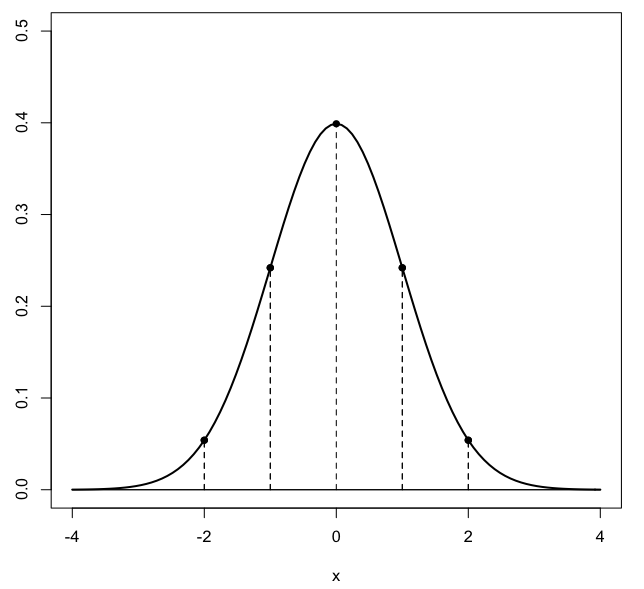
\includegraphics [scale=0.4] {gauss3.png} \end{center}

%break
\title{Maximum likelihood}
\date{}

\begin{document}
\maketitle
\Large
    
A nice application of logarithmic differentiation is of a set of Bernoulli trials, like a series of coin flips where the coin isn't fair, but instead has a probability $p$ of coming up heads (H) and $1-p$ of coming up tails (T).

Note that this classic example is actually impossible to achieve.  One cannot "weight" a coin to do this, though it is easy with a die (singular of dice).

\url{http://www.stat.columbia.edu/~gelman/research/published/diceRev2.pdf}

Now, $p$ is unknown, but we have some data about how the coin performs, and we wish to use the data to estimate $p$ by the method of maximum likelihood.  We observe this sequence of trials:
\[  HTHHTTTHTHHH  \]

Theory says that the probability of observing this sequence of events is dependent on $p$ in the following way:
\[  p(1-p)pp(1-p)(1-p)(1-p)p(1-p)ppp = p^7(1-p)^5  \]

We call the probability of observing this data, given some underlying probability model $p$, the likelihood $L$:
\[  L(p) = p^7(1-p)^5  \]
(It's called the likelihood, because the total probability is not equal to $1$).

In general, since each trial is independent and identically distributed

\url{https://en.wikipedia.org/wiki/Independent_and_identically_distributed_random_variables}

we can write that for $n$ trials and $k$ successes we would have
\[  L(p) = p^k(1-p)^{n-k}  \]

Here, $n$ and $k$ are constants for any particular sequence, but we would like to have the general formula.
 
To find the maximum for $L$ we differentiate and set that equal to 0.
\[  \frac{d}{dp} L = 0  \]

However, we note that since $\ln L$ increases and decreases along with $L$, the value of $p$ that gives a maximum for $L$ also gives a maximum for $\ln L$.  So we will take the logarithm of $L$ and set that equal to zero:
\[  \frac{d}{dp} \ln L = 0  \]
\[  \ln L = k \ln p + (n-k) \ln(1-p)  \]

Take the derivative $d/dp$ of both sides (we get a minus sign from the chain rule):
\[  \frac{d}{dp} \ln L = 0 = \frac{k}{p} - \frac{n-k}{1-p}  \]
\[   \frac{k}{p} = \frac{n-k}{1-p}  \]

Multiply through by $1-p$ and also by $1/k$:
\[  \frac{1-p}{p} = \frac{n-k}{k}  \]
\[   \frac{1}{p} = \frac{n}{k}  \]
\[    p = \frac{k}{n}  \]

As we might have guessed, the maximum likelihood estimate of $p$ is simply the ratio of the observed number of successes to the number of trials:  $k/n$.
\end{document}